
\paragraph{} This chapter will cover a number of topics essential to understanding the rationale and implementation of the design as discussed in §~\ref{sec:design}. These include; Intel SGX, a brief overview of modern \textit{libOSes}, an introduction to \textit{Information Flow Control} (\textit{IFC}), and a overview of key aspects of the Linux kernel relevant to the architecture of the prototype.

\section{Intel SGX}

\paragraph{} Intel's Software Guard Extensions, SGX, was first announced and detailed in a handful of whitepaper documents published in 2013. [X,Y,Z] It described a novel approach, creating in-CPU containers with their own protected memory pools. These regions, called \textit{enclaves}, cannot be read from or written to by an unauthorised party due to fundamental protection mechanisms provided by the x86 architecture, even if running in \textit{Ring 0}:\footnote{x86 offers four protection \textit{rings}, of which Linux uses two --- \textit{0} for the kernel, and \textit{3} for userspace.} Figure~\ref{fig:sgx-basic} illustates this. \textit{Enclaves} guarantee both integrity and secrecy to the application running inside it, even in the prescence of a malicious host.

\paragraph{Motivation} At a high level SGX aims to achieve security for sensitive application by shielding them, and the resources it uses, against tampering and to provide a guarantee to end users about an enclave's integrity; this is achieved using attestation (§~\ref{sec:attestation}) and measurement (§~\ref{sec:provisioning}). A driving use case is in a cloud computing context, where users are forced to trust a foreign party with both their data and business logic. By distributing encrypted, yet executable, containers targetting a single, unique SGX core, users can be assured that their information is safe, regardless of any virutalisation that may be taking place. Only the provisioned CPU is able to decrypt and execute the enclave, strictly in accordance with the restrictions of the SGX platform.

\subsection{Security Characteristics}

\begin{figure}[]
    \centering
    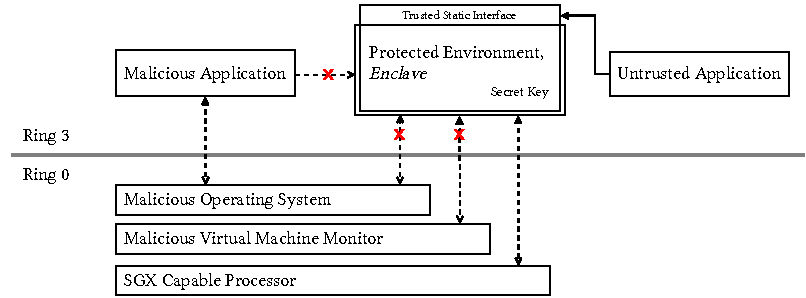
\includegraphics[width=0.95\linewidth]{figures/SGX-architecture.pdf}
    \caption{Abstract overview of SGX's protection in an adversarial environment.}
    \label{fig:sgx-basic}
\end{figure}

\paragraph{} At its heart SGX is designed to be \textit{trustworthy}; this is achieved in a number of ways, including robust enclaving provisioning, sealing and attestation. Intel enumerates SGX's protections as follows;

\begin{itemize}
    \item Memory security against observation and modification from outside the enclave; this is achieved using an in-die \textit{Memory Encryption Engine} (\textit{MEE}), with a secret that rotates on every boot. This protection notably works against a host hypervisor, other enclaves, and anything running in supervisor mode.
    \item Attestation of an enclave to a challenger through the use of a permanent hardware security key for asymmetric encryption.
    \item Proxied software calls to prepare and transfer control in and out of an enclave. Arguments are securely marshalled according to a static enclave definition.
    \item SGX does not defend against reverse engineering or sidechannel attacks: [X,Y] this is the responsibility of the developer to mitigate.
    \item Debugging support is only provided via a specialised tool and only when an enclave is compiled with debugging enabled.
\end{itemize}

\subsection{Architecture and Implementation}

\begin{figure}[]
    \centering
    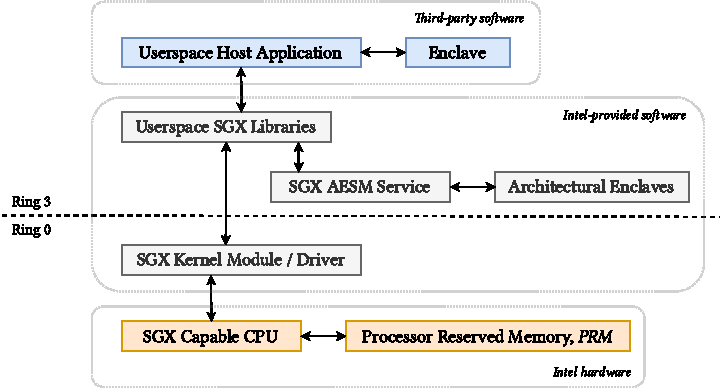
\includegraphics[width=0.9\linewidth]{figures/SGX-AdvArchitecture.pdf}
    \caption{A high-level overview of the SGX hardware and software architecture.}
    \label{fig:sgx-advarch}
\end{figure}

\paragraph{} The SGX platform comprises a number of interlocking parts, as shown in Figure~\ref{fig:sgx-advarch}. Working from the hardware up, at the heart of the platform is the extended x86 instruction set and memory protection provided by an SGX-capable CPU. 

\paragraph{Hardware} Enclaves' data and code is stored securely in \textit{Processor Reserved Memory}, \textit{PRM}; this is a set of pages in system memory that are presided over by the \textit{MEE}. DMA\footnote{Direct Memory Access} to \textit{PRM} is always rejected. \textit{PRM} consists of two datastructures; the \textit{Enclave Page Cache Map} (\textit{EPCM}) and the \textit{Enclave Page Cache} (\textit{EPC}). An individual enclave is defined by an \textit{SGX Enclave Control Structure}, \textit{SECS}; this is generated when an enclave is created and stored in a dedicated entry in the \textit{EPC}. An enclave's \textit{SECS} contains important information such as its (system) global identifier, its measurement hash and the amount of memory it is using. Access control information is stored in the \textit{EPCM} alongside page validity flags, the owning enclave identifier and the page's type; this is not accessible from software. An attempt to resolve a page in \textit{PRM} is successful only if the CPU is executing in enclave mode and its \textit{EPCM} entry states it belongs the currently executing enclave --- if this is not the case the lookup returns an unused page from generic system memory.

\paragraph{} The host OS or hypervisor manages the \textit{EPC} just as it does with normal system memory, swapping pages in and out according to its own policy, but must do so using SGX specific instructions. The \textit{MEE} is responsible for ensuring the integirty and confidentiality of this process, encrypting and decrypting pages as they cross the \textit{PRM} boundary. Data is verified with the use of an integrity tree, and encryption keys are generated at boot-time. Importantly the SGX archicture relies on the host OS being SGX-aware, empowering userspace applications to function without privilege; this is provided by the SGX driver, \textit{isgx}.

\paragraph{Userspace services} Starting an enclave requires retrieving a \textit{launch token} from Intel's \textit{Launch Enclave}; this checks the signature and identity of the enclave to ensure it is valid. Access to the \textit{Launch Enclave} and other architectural enclaves is provided by the AESM service; the userspace SGX libraries facilitate the communication mechanism. Other architectural enclaves include;

\begin{itemize}
    \item The \textit{Provisioning Enclave} --- this verifies the authenticity of the platform and retrieves an enclave's \textit{attestation key} from the \textit{Intel Provisioning Service's} servers.
    \item The \textit{Quoting Enclave} --- this provides trust in the identity of the SGX environment and enclave being attested, by converting the locally generated \textit{attestation key} to a remotely-verifiable \textit{quote}.
\end{itemize}

\paragraph{Third-party enclaves} Enclaves can only be entered via userspace, as detailed in §~\ref{sec:sgx-lifecycle}, and are always accompanied by a host application which acts as its untrusted counterpart. The host application calls the SGX SDK to build an enclave on its behalf using an enclave image, packaged as a standard shared library (\texttt{enclave.so}) and returns its \textit{global identifier}. Control is passed from the host application to the enclave by invoking an enclave function via an \textit{ECALL}. Execution flow can temporarily leave the enclave if it call one of the host application's function via an \textit{OCALL}. Execution naturally leaves enclave-mode when the \textit{ECALL} terminates. Both \textit{ECALLs} and \textit{OCALLs} are defined statically in the enclave's interface definition (\texttt{enclave.edl}). The necessary glue code is generated by the SGX SDK's build toolchain at compile time; this ensures calls crossing the enclave boundary are marshalled safely and correctly.


\subsection{Enclave Lifecycle}
\label{sec:sgx-lifecycle}

\paragraph{} SGX instructions can be separated into two distinct groups; privileged and unprivileged. These, alongside a description of the function they perform, are enumerated in Table~\ref{table:sgx-instructions}.\footnote{A handful of instructions not relevant to the explanation given here are omitted.} The following description of the process of creating an enclave is illustrated in Figure~\ref{fig:sgx-enclavecreate}.

\paragraph{Preparing an enclave} Execution begins with the host application; is needs to initiate the creation process, but must do so via a component with \textit{Ring 0} privilege. This facility is provided by \textit{isgx}, the SGX driver. The application first requests \textit{isgx} to allocate the necessary number of pages to run the enclave $\langle 1 \rangle$;\footnote{These numbers correspond to events in Figure~\ref{fig:sgx-enclavecreate}.} this is tracked and served from the driver's internal state $\langle 2 \rangle$.

\paragraph{} The application continues by executing \texttt{ECREATE} with the metadata of the enclave to be loaded $\langle 3 \rangle$; the \textit{MEE} checks that the pages being claimed are in fact vacant and populates the \textit{SECS} page with the necessary information $\langle 4 \rangle$. Once this is complete the application prepares the remaining \textit{EPC} pages using \texttt{EADD} $\langle 5 \rangle$ and loads the enclave's code and data $\langle 6 \rangle$.

\paragraph{} At this point the enclave needs to be measured --- the application calls \texttt{EEXTEND} $\langle 7 \rangle$, triggering the \textit{MEE} to update the measurement hash in the \textit{SECS} to aligns with the current state of the enclave's memory $\langle 8 \rangle$. Once the \textit{EPC} memory is prepared the applications requests for it to be finalised using \texttt{EINIT} $\langle 9 \rangle$: this operation requires the application to retrieve the \texttt{EINITTOKEN} from the \textit{Launch Enclave}, locking the execution of the measured enclave to the CPU the token is generated on. Notably, pages cannot be added after \texttt{EINIT},\footnote{This is only strictly true in SGXv1, as explained in §~\ref{sec:sgx-versions}.} and an enclave cannot be attested to or entered before it. Finally, the initialised flag is set in the \textit{SECS} and the enclave's hash updated for the final time $\langle 10 \rangle$.


\begin{figure}[]
    \centering
    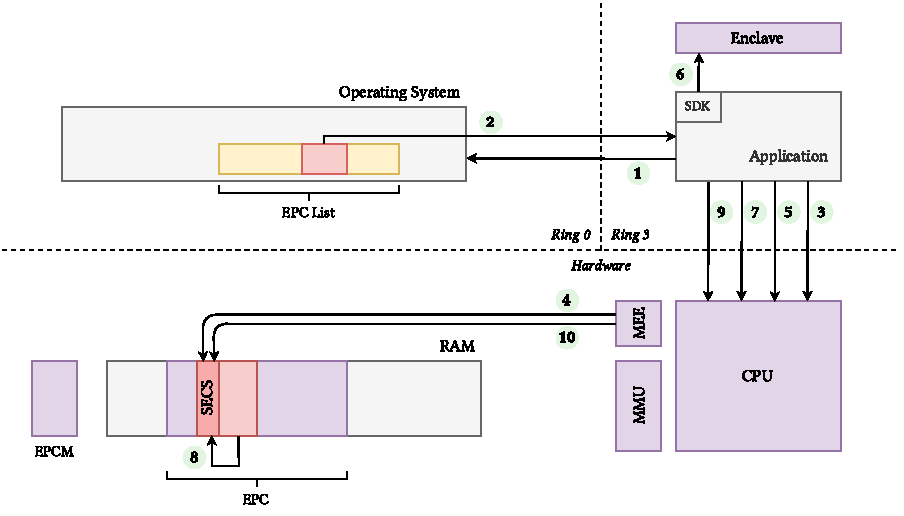
\includegraphics[width=\linewidth]{figures/SGX-EnclaveCreate.pdf}
    \caption{The process of creating and initialising an enclave; details given in §~\ref{sec:sgx-lifecycle}. Purple components belong to the SGX platform.}
    \label{fig:sgx-enclavecreate}
\end{figure}

\paragraph{Stepping into the enclave} Once an enclave is created is can be invoked using the \texttt{EENTER} instruction. This can only jump to code explicitly defined in the enclave's interface definition and switches the CPU core to enclave mode. SGX uses a flag in the CPU core's \textit{Thread Control Block} to prevent any other logical core following the current one into the enclave.

\paragraph{} Interrupts and exceptions can be served to the enclave, just as with any other application. When in enclave mode control is not immediately passed over to the defined handler, but instead the enclave's current state is saved and cleared to ensure no data is leaked. The \textit{Asynchronous Enclave Exit} routine is then invoked and enclave mode disabled. Execution post-interruption is restarted with the \texttt{ERESUME} instruction. Once an enclave has finished executing the registers are erased and \texttt{EEXIT} called. Enclaves are terminated using the \texttt{EREMOVE} command; all claimed \textit{EPC} pages are marked as invalid and the \textit{SECS} page deleted.

\paragraph{} \label{sec:sgx-no-kernel-mode} A significant design decision made in the SGX architecture is that enclaves cannot be entered by a process operating in \textit{Ring 0}; the required instructions simply aren't available. This forces all host applications to run in userspace, making interoperation with the kernel challenging, as will be discussed in §~\ref{sec:design}.

\begin{table}
    \centering
    \newcommand\tableTop{\rule{0pt}{3ex}}
    \newcommand\tableMid{\rule{0pt}{3ex}}
    \newcommand\tableBottom{\rule[-2ex]{0pt}{0pt}}
    \begin{tabular}{|c|r|p{8.5cm}|} 
        \hline
        Execution Mode & Instruction & Function \\ [0.1ex] 
        \hline\hline
        \multirow{11}{*}{Ring 0} 
            & \tableTop{\texttt{ECREATE}} & \tableTop{Generate and copy the \textit{SECS} structure to a new page in the \textit{EPC}, initialising a new enclave.} \\ 
            & \texttt{EADD} & \tableMid{Add a new \textit{EPC} page for the current enclave; this is used to load initial code and data.} \\ 
            & \texttt{EEXTEND} & \tableMid{Updates the enclave's measurement during attestation; modifies the \textit{SECS}.} \\ 
            & \texttt{EINIT} & \tableMid{The terminal instruction in an enclave's initialisation, finalising its attributes and measurement.} \\ 
            & \texttt{EREMOVE} & \tableMid{Permanently remove a page from the \textit{EPC}; usually invoked during enclave destruction.} \tableBottom \\ 
        \hline\hline
        \multirow{11}{*}{Ring 3} 
        & \tableTop{\texttt{EENTER}} & \tableTop{Transfer control from the host application to a pre-determined location in an enclave.} \\ 
        & \texttt{ERESUME} & \tableMid{Re-enter the enclave after an interrupt/exception and resume execution.} \\ 
        & \texttt{EEXIT} & \tableMid{Restore the original operating mode at the location \texttt{EENTER} was triggered and flush the TLB.} \\ 
        & \texttt{EGETKEY} & \tableMid{Access platform cryptography keys required for attestation and sealing.} \\ 
        & \texttt{EREPORT} & \tableMid{Generate a \textit{report} for an enclave's \textit{attestation key} for an attestation process.} \tableBottom \\ 
        \hline
    \end{tabular}
    \vspace{5mm}
    \caption{Overview of notable SGX x86 instructions in an enclave's lifecycle.}
    \label{table:sgx-instructions}
\end{table}


\subsection{Attestation}
\label{sec:attestation}

\paragraph{} An essential feature of the \textit{trusted computing} model SGX creates is attestation, the process of verifying both the authenticity and integrity of component cryptographically. SGX achieves by creating two hashed values, or \textit{signing identifies}, per enclave; \texttt{MRENCLAVE} and \texttt{MRSIGNER}.

\paragraph{} \texttt{MRENCLAVE} acts an a unique identifier for the contents of an enclave. It is generated by hashing the instructions and data passed when creating the enclave with \texttt{ECREATE}, \texttt{EADD}, and \texttt{EEXTEND}; the value is finalised and stored in the \textit{SECS} on \texttt{EINIT}. This values depends on the exact content and ordering of the enclave's \textit{EPC} pages. As long as the enclave's source remains the same, so will its \texttt{MRENCLAVE}.

\paragraph{} \texttt{MRSIGNER}, also known as the enclave's \textit{Sealing Identity}, is generated during the enclave build process --- all production enclaves need to be signed using an RSA key provided by the compiling user (the \textit{Sealing Authority}). The public key from this pair is stored in \textit{SIGSTRUCT}, the \textit{Enclave Signature Structure}. During an enclave's launch its \textit{SIGSTRUCT}, which holds the signed compile-time \texttt{MRENCLAVE} value, is decrypted and crossreferenced with a freshly-computed runtime \texttt{MRENCLAVE} value to detect tampering. \texttt{MRSIGNER} is the same for all enclaves signed by the same \textit{Sealing Authority}.

\paragraph{Local Attestation} Two enclaves reisdent on the same system are able to attest their identities to each other using their \texttt{MRENCLAVE} and \texttt{MRSIGNER} values; this usually precedes the establishment of a shared secret (using a variant of \textit{Diffie-Hellman} backed by the platform's master SGX key)\footnote{Note for Harri: must check these details.} for confidential communication between them.

\paragraph{Remote Attestation} In addition to attestation between entities on the same platform, the Intel specifiation also provides a workflow for an enclave to attest its identity to a remote party. The system's \textit{Quoting Enclave} verifies an enclave's local \textit{quote} and creates a digital signature of it using the CPU's permanent hardware SGX private key. Through the use of an \textit{Intel Enchanced Privacy Identifier} (\textit{EPID}) this process can be carried out anonymously; it relies on information encoded in the CPU during the manufacturing process. The \textit{Provisioning Enclave} assists in this process, especially as production enclaves are required to attest with Inthel's provisioning service before executing. Remote attestation is not explicitly required in this project's architecture hence will not be covered in any further detail.

\subsection{Provisioning and Sealing}
\label{sec:provisioning}

\subsection{SGX Versions}
\label{sec:sgx-versions}

\section{Modern \textit{libOSes}}

\section{Information Flow Control}

\section{Aspects of the \textit{Linux} Kernel}